\section{Architecture}
In Figure \ref{fig:modelDiagram} it is shown the general diagram of the packages 
\begin{figure}[!h]
	\centering
	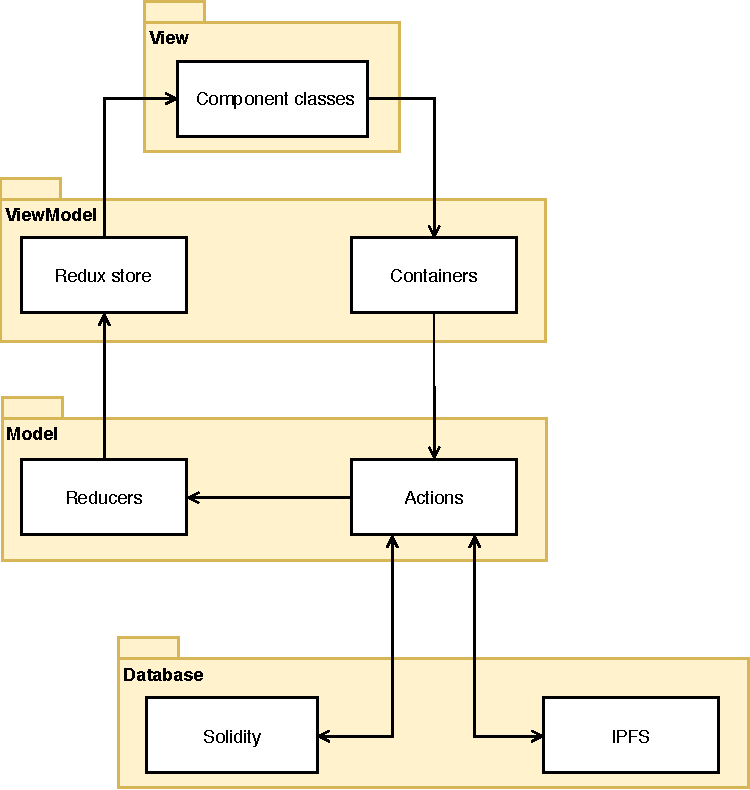
\includegraphics[height=3in]{img/generalPackageDiagram.pdf}
	\caption{The general diagram of the packages}
	\label{fig:modelDiagram}
\end{figure}
\subsubsection{View, Model and ViewModel}
The View contains all the React components. Those classes do not have any bound with the reducer store. They are imported by the containers, which are in the ViewModel part. The containers together with the store are responsible of the communications between the components and the actions, which are part of the Model part. The Model takes care of making the requests to the server(s) and to dispatch the information back to the store.
Please refer to the \verb|ViewDiagram.pdf|, \verb|ViewModelDiagram.pdf| and the \verb|ModelDiagram.js| in the \verb|attachment| folder to understand more deeply how they are organized in detail.
 